%!TEX root = ../TaxationPlan.tex

In this appendix, we plot all of the graphs from the numerical section for alternative
parameterizations.

\newpage
\clearpage
\subsection{Fluctuating $r$}

In this section, we consider three alternative values for the risk-free rate

\subsubsection{Graphs with $r \approx 0.01$ (annualized)}

  \begin{center}
    \begin{figure}[H]
      \scalebox{0.65}{\includegraphics{./TaxationPlanImages/model_15575839184342234450/StochasticMarginGrowth.png}}
    \end{figure}
  \end{center}

  \begin{center}
    \begin{figure}[H]
      \scalebox{0.65}{\includegraphics{./TaxationPlanImages/model_15575839184342234450/AnnualizedBuybacks.png}}
    \end{figure}
  \end{center}

  \begin{center}
    \begin{figure}[H]
      \scalebox{0.65}{\includegraphics{./TaxationPlanImages/model_15575839184342234450/AnnualizedTaxRates.png}}
    \end{figure}
  \end{center}

  \begin{center}
    \begin{figure}[H]
      \scalebox{0.45}{\includegraphics{./TaxationPlanImages/model_15575839184342234450/SimulationPlots.png}}
    \end{figure}
  \end{center}

\newpage
\clearpage
\subsubsection{Graphs with $r \approx 0.05$ (annualized)}

  \begin{center}
    \begin{figure}[H]
      \scalebox{0.65}{\includegraphics{./TaxationPlanImages/model_998767372562120623/StochasticMarginGrowth.png}}
    \end{figure}
  \end{center}

  \begin{center}
    \begin{figure}[H]
      \scalebox{0.65}{\includegraphics{./TaxationPlanImages/model_998767372562120623/AnnualizedBuybacks.png}}
    \end{figure}
  \end{center}

  \begin{center}
    \begin{figure}[H]
      \scalebox{0.65}{\includegraphics{./TaxationPlanImages/model_998767372562120623/AnnualizedTaxRates.png}}
    \end{figure}
  \end{center}

  \begin{center}
    \begin{figure}[H]
      \scalebox{0.45}{\includegraphics{./TaxationPlanImages/model_998767372562120623/SimulationPlots.png}}
    \end{figure}
  \end{center}

\newpage
\clearpage
\subsubsection{Graphs with $r \approx 0.10$ (annualized)}

  \begin{center}
    \begin{figure}[H]
      \scalebox{0.65}{\includegraphics{./TaxationPlanImages/model_13340340551259069813/StochasticMarginGrowth.png}}
    \end{figure}
  \end{center}

  \begin{center}
    \begin{figure}[H]
      \scalebox{0.65}{\includegraphics{./TaxationPlanImages/model_13340340551259069813/AnnualizedBuybacks.png}}
    \end{figure}
  \end{center}

  \begin{center}
    \begin{figure}[H]
      \scalebox{0.65}{\includegraphics{./TaxationPlanImages/model_13340340551259069813/AnnualizedTaxRates.png}}
    \end{figure}
  \end{center}

  \begin{center}
    \begin{figure}[H]
      \scalebox{0.45}{\includegraphics{./TaxationPlanImages/model_13340340551259069813/SimulationPlots.png}}
    \end{figure}
  \end{center}

\newpage
\clearpage
\subsection{Fluctuating $\gamma$}

In this section, we consider two alternative values for the percent of margin that can be seized.

\subsubsection{Graphs with $\gamma = 0.75$}

  \begin{center}
    \begin{figure}[H]
      \scalebox{0.65}{\includegraphics{./TaxationPlanImages/model_13157355545147574999/StochasticMarginGrowth.png}}
    \end{figure}
  \end{center}

  \begin{center}
    \begin{figure}[H]
      \scalebox{0.65}{\includegraphics{./TaxationPlanImages/model_13157355545147574999/AnnualizedBuybacks.png}}
    \end{figure}
  \end{center}

  \begin{center}
    \begin{figure}[H]
      \scalebox{0.65}{\includegraphics{./TaxationPlanImages/model_13157355545147574999/AnnualizedTaxRates.png}}
    \end{figure}
  \end{center}

  \begin{center}
    \begin{figure}[H]
      \scalebox{0.45}{\includegraphics{./TaxationPlanImages/model_13157355545147574999/SimulationPlots.png}}
    \end{figure}
  \end{center}

\newpage
\clearpage
\subsubsection{Graphs with $\gamma = 0.90$}

  \begin{center}
    \begin{figure}[H]
      \scalebox{0.65}{\includegraphics{./TaxationPlanImages/model_12582278578111521445/StochasticMarginGrowth.png}}
    \end{figure}
  \end{center}

  \begin{center}
    \begin{figure}[H]
      \scalebox{0.65}{\includegraphics{./TaxationPlanImages/model_12582278578111521445/AnnualizedBuybacks.png}}
    \end{figure}
  \end{center}

  \begin{center}
    \begin{figure}[H]
      \scalebox{0.65}{\includegraphics{./TaxationPlanImages/model_12582278578111521445/AnnualizedTaxRates.png}}
    \end{figure}
  \end{center}

  \begin{center}
    \begin{figure}[H]
      \scalebox{0.45}{\includegraphics{./TaxationPlanImages/model_12582278578111521445/SimulationPlots.png}}
    \end{figure}
  \end{center}

\newpage
\clearpage
\subsection{Fluctuating $\hat{\tau}$}

In this section, we consider three alternative values for the baseline fee amount

\subsubsection{Graphs with $\hat{\tau} \approx 0.02$ (annualized)}

  \begin{center}
    \begin{figure}[H]
      \scalebox{0.65}{\includegraphics{./TaxationPlanImages/model_9802577656585622608/StochasticMarginGrowth.png}}
    \end{figure}
  \end{center}

  \begin{center}
    \begin{figure}[H]
      \scalebox{0.65}{\includegraphics{./TaxationPlanImages/model_9802577656585622608/AnnualizedBuybacks.png}}
    \end{figure}
  \end{center}

  \begin{center}
    \begin{figure}[H]
      \scalebox{0.65}{\includegraphics{./TaxationPlanImages/model_9802577656585622608/AnnualizedTaxRates.png}}
    \end{figure}
  \end{center}

  \begin{center}
    \begin{figure}[H]
      \scalebox{0.45}{\includegraphics{./TaxationPlanImages/model_9802577656585622608/SimulationPlots.png}}
    \end{figure}
  \end{center}

\newpage
\clearpage
\subsubsection{Graphs with $\hat{\tau} \approx 0.004$ (annualized)}

  \begin{center}
    \begin{figure}[H]
      \scalebox{0.65}{\includegraphics{./TaxationPlanImages/model_17012022837339294945/StochasticMarginGrowth.png}}
    \end{figure}
  \end{center}

  \begin{center}
    \begin{figure}[H]
      \scalebox{0.65}{\includegraphics{./TaxationPlanImages/model_17012022837339294945/AnnualizedBuybacks.png}}
    \end{figure}
  \end{center}

  \begin{center}
    \begin{figure}[H]
      \scalebox{0.65}{\includegraphics{./TaxationPlanImages/model_17012022837339294945/AnnualizedTaxRates.png}}
    \end{figure}
  \end{center}

  \begin{center}
    \begin{figure}[H]
      \scalebox{0.45}{\includegraphics{./TaxationPlanImages/model_17012022837339294945/SimulationPlots.png}}
    \end{figure}
  \end{center}

\newpage
\clearpage
\subsubsection{Graphs with $\hat{\tau}= 0.0001$ (annualized)}

  \begin{center}
    \begin{figure}[H]
      \scalebox{0.65}{\includegraphics{./TaxationPlanImages/model_9527164782035243315/StochasticMarginGrowth.png}}
    \end{figure}
  \end{center}

  \begin{center}
    \begin{figure}[H]
      \scalebox{0.65}{\includegraphics{./TaxationPlanImages/model_9527164782035243315/AnnualizedBuybacks.png}}
    \end{figure}
  \end{center}

  \begin{center}
    \begin{figure}[H]
      \scalebox{0.65}{\includegraphics{./TaxationPlanImages/model_9527164782035243315/AnnualizedTaxRates.png}}
    \end{figure}
  \end{center}

  \begin{center}
    \begin{figure}[H]
      \scalebox{0.45}{\includegraphics{./TaxationPlanImages/model_9527164782035243315/SimulationPlots.png}}
    \end{figure}
  \end{center}
